\documentclass[11pt,a4paper]{article}
\usepackage[latin5]{inputenc}
\usepackage[english]{babel}
\usepackage{amsmath}
\usepackage{amsfonts}
\usepackage{amssymb}
\usepackage{graphicx,subfig}
\usepackage{placeins}
\usepackage{gensymb}

\author{Alexander Attinger, Yannic Kilcher}
\title{Report Blatt 4, Advanced Part}

\begin{document}
\maketitle

\section{Watershed segmentation}
We were asked to perform a watershed segmentation on a preprocessed image. We have done the preprocessing with the provided image of apples, as seen in Fig. \ref{fig:e1}
\begin{figure}

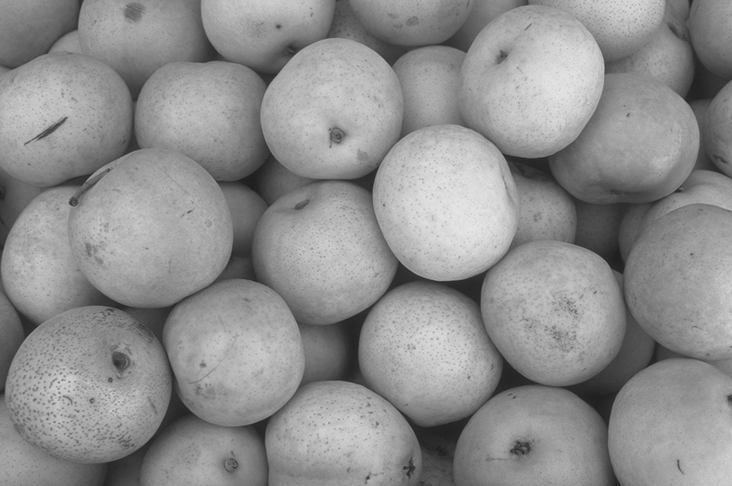
\includegraphics[scale=.5]{data/res/adv/apples.png}
\caption{The original Image}%
\label{fig:e1}
\end{figure}

After the preprocessing, which consisted of various morphological operations, we could obtain a foreground and background label map. We combined these to give us a single label map to give to the watershed algorighm. In this map, as seen in Fig. \ref{fig:e2}, foreground pixels are labeled with intensity 255, background pixels are labeled with intensity 155 and unknown pixels are labeled with intensity 0.

\begin{figure}
\centering
\subfloat[][Disk radius 2]{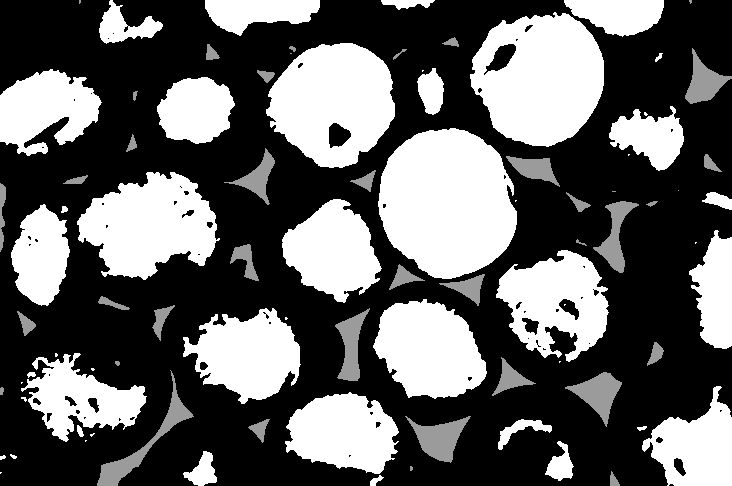
\includegraphics[scale=.3]{data/res/adv/label_map_2.png}}
\quad
\subfloat[][Disk radius 10]{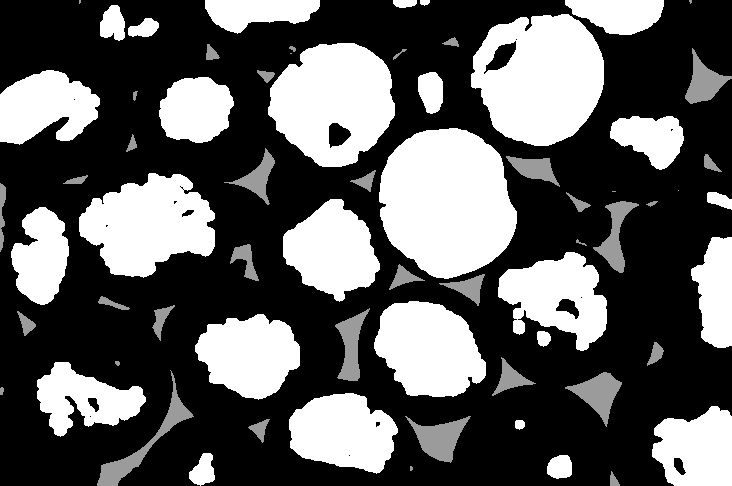
\includegraphics[scale=.3]{data/res/adv/label_map_10.png}}
\quad
\subfloat[][Disk radius 20]{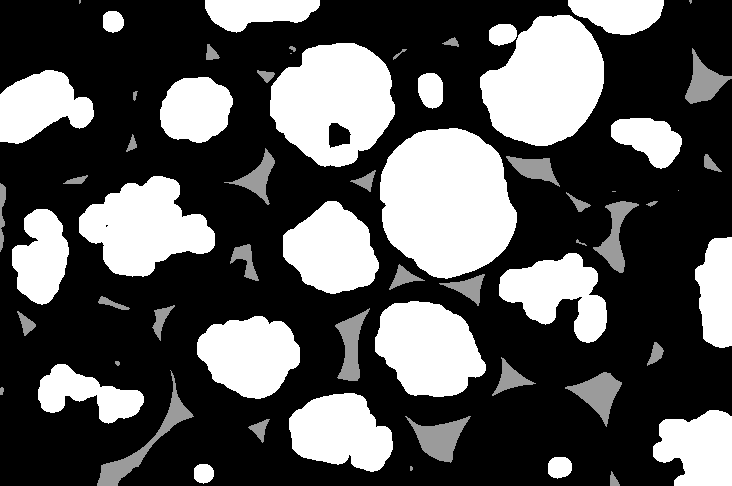
\includegraphics[scale=.3]{data/res/adv/label_map_20.png}}
\quad
\subfloat[][Disk radius 50]{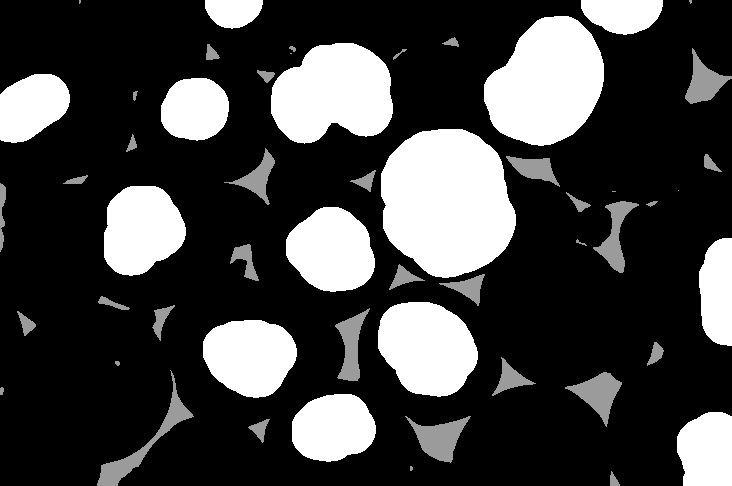
\includegraphics[scale=.3]{data/res/adv/label_map_50.png}}
\quad

\caption{Label maps with various morphological operator sizes. Foreground thresholding at 160, background thresholding at 60}%
\label{fig:e2}
\end{figure}

The watershed algorithm iteratively fills the unknown pixels by expanding the already known regions. After the algorithm, we obtain the final label map, shown in Fig. \ref{fig:e3}.

\begin{figure}
\centering
\subfloat[][Disk radius 2]{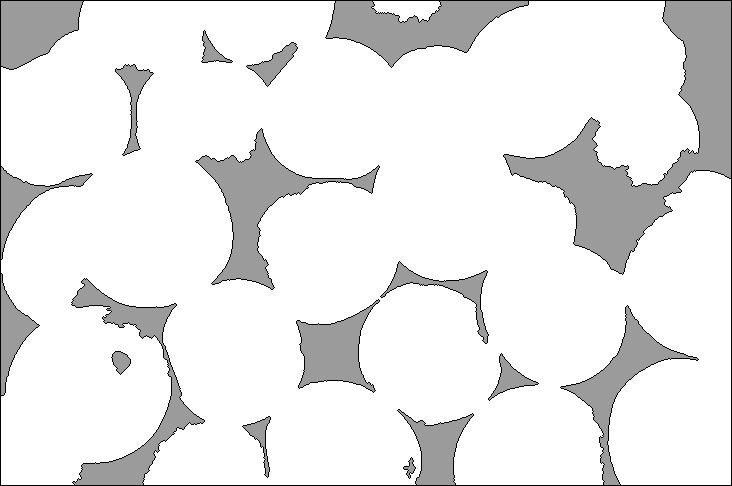
\includegraphics[scale=.3]{data/res/adv/markers_after_2.png}}
\quad
\subfloat[][Disk radius 10]{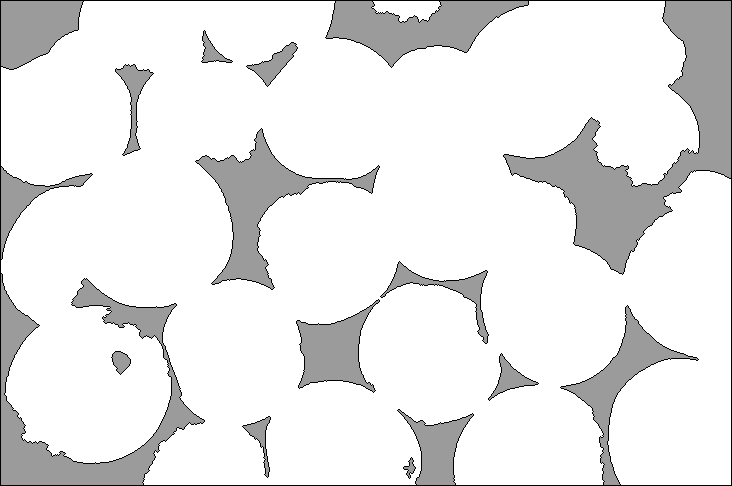
\includegraphics[scale=.3]{data/res/adv/markers_after_10.png}}
\quad
\subfloat[][Disk radius 20]{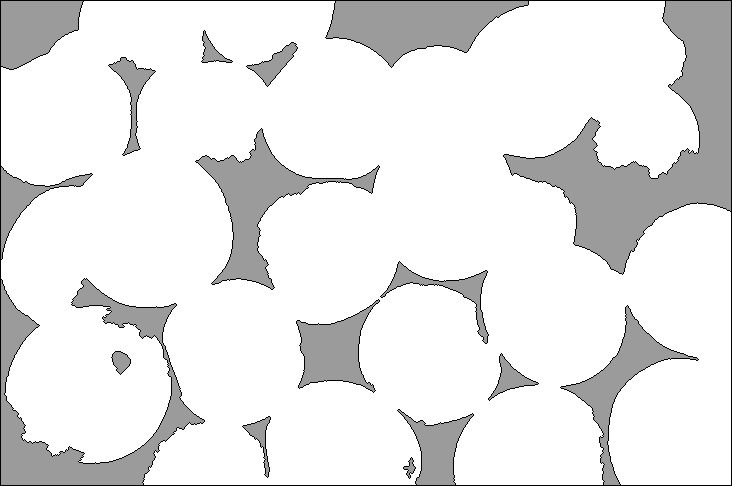
\includegraphics[scale=.3]{data/res/adv/markers_after_20.png}}
\quad
\subfloat[][Disk radius 50]{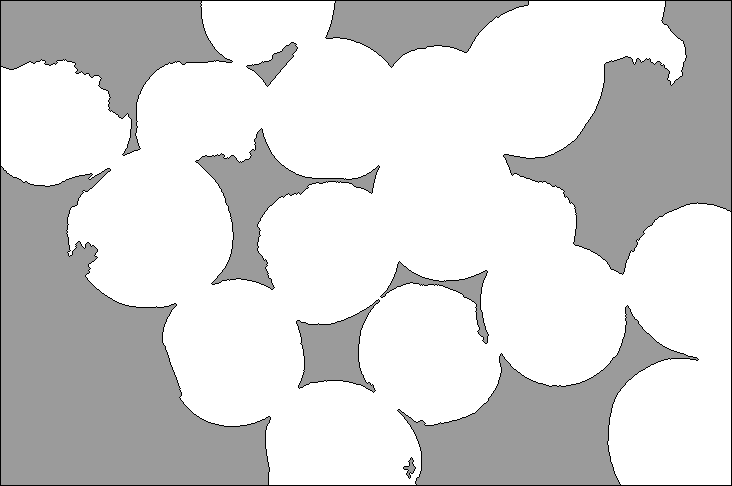
\includegraphics[scale=.3]{data/res/adv/markers_after_50.png}}
\quad

\caption{Final label maps with various morphological operator sizes.}%
\label{fig:e3}
\end{figure}

As one can see, the algorithm selects more apples to the foreground, the smaller the initial disk radius, which is mainly due to more apples being labeled as foreground in the initial foreground map, which in turn results from the smaller disk size being able to "fit into" more parts of the apples.\\
The watershed algorighm generally performs well, but a big problem is that once something is labeled as a certain region, the label will not change. This is problematic, when one cannot reasonably threshold it out in the initial label maps, as is the case with the middle part of an apple on the bottom left being labeled as background right from the start, which will never change.

\FloatBarrier

\end{document}

